\documentclass[12pt,letterpaper]{article}

\usepackage[spanish]{babel}
\usepackage[utf8]{inputenc}
\usepackage{graphicx}
\usepackage{pst-pdf}
\usepackage{amssymb}
\usepackage{hyperref}
\usepackage{listings}
\usepackage[backend=bibtex,sorting=none]{biblatex}
\bibliography{bibliography}

\title{Proyecto}
\author{Mariela López Jarquín}
\date{\today}

\begin{document}
\maketitle
\abstract{A continuación se muestra la programación del algoritmo para calcular la transformada de Fourier, la DFT (Transformada de Fourier Discreta) y FFT (Transformada rápida de Fourier). }

\section{Transformada de Fourier Discreta}
La transformada discreta de Fourier o DFT es un tipo de transformada discreta utilizada en el análisis de Fourier. Transforma una función matemática en otra, obteniendo una representación en el dominio de la frecuencia, siendo la función original una función en el dominio del tiempo. \\

La secuencia de $N$ n\'umeros complejos $ x_0 , ..., x_{N-1} $ se transforma en la secuencia de $N$ n\'umeros complejos $ X_0 , ..., X_{N-1} $ mediante la DFT con la f\'ormula
$$
 X(k) = \sum_{n=0}^{N-1} x(n) e ^ {- \frac{i2\pi}{N}kn} \ \ \ \ \ \ \ k = 0,..., N-1
$$

\subsection{Problema computacional.}
\textbf{Objetivo:} Calcular la transformada de fourier da una funci\'on.

\textbf{Entrada:} El n\'umero n representa la cantidad de muestras.

\textbf{Salida:} El tiempo de ejecuci\'on de cada n muestra.

\subsection{Algoritmo.}
Para el algoritmo se utiliz\'o $f(x) = 2sin(2 \pi x) + 5cos(2 \pi x) $ y también se us\'o la libreria complex para manipular n\'umeros complejo. El C++ tiene una potente librería standard para numeros complejos. Se puede utilizar incluyendo en la libreria del programa $#$ $include <complex>$

\subsection{Instancia del problema.}
Como prueba de escritorio, se seleccion\'o la siguiente instancia del problema. Entrada: $4096$. La salida del programa se observa en la Figura 1.

\begin{figure}[ht!]
  \centering
  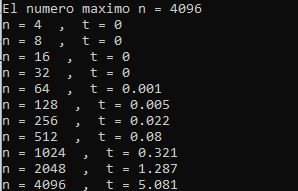
\includegraphics[width=0.8\textwidth]{D}
  \caption{Ejecución del programa.}
  \label{fig:FFT_1d}
\end{figure}

\section{Transformada Rápida de Fourier}
Conocida por la abreviatura FFT es un algoritmo eficiente que permite calcular la transformada de Fourier discreta y su inversa. Su importancia radica en el hecho que elimina una gran parte de los c\'alculos repetitivos a que est\'a sometida la DFT, por lo tanto se logra un c\'alculo m\'as r\'apido.

\subsection{Problema computacional.}
\textbf{Objetivo:} Calcular la transformada de fourier mediante Transformada Rápida de Fourier.

\textbf{Entrada:} El valor de n para la cantidad de muestra.

\textbf{Salida:} El tiempo de ejecuci\'on de cada n muestra.

\subsection{Algoritmo.}
Al igual que el DFT se utiliz\'o la misma funci\'on de prueba y mismas librerias junto con los metodos de la clase Complex para la programaci\'on del algoritmo FFT.

\subsection{Instancia del problema.}
Como prueba de escritorio, se seleccion\'o la siguiente instancia del problema. Entrada: $8192$, el cual es significativamente mayo que la instancia en el DFT ya que el algoritmo FFT es mucho m\'as eficiente. La salida del programa se observa en la Figura 2. \\

\begin{figure}[ht!]
  \centering
  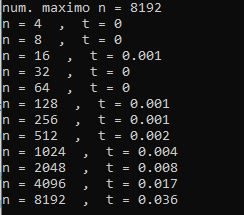
\includegraphics[width=0.8\textwidth]{FFT}
  \caption{Ejecución del programa.}
  \label{fig:FFT}
\end{figure}

\newpage

\section{Comparaci\'on entre DFT y FFT}
Comparando los datos de tiempo de ejecuci\'on por cada $n$ muestra entre el DFT y FFT notamos una gran diferencia entre tiempos de ejecuci\'on, lo cual tiene sentido ya que el algoritmo de DFT se utiliz\'an dos ciclos for uno dentro de otro de tamaño de iteraci\'o $n$. Por otra parte el algoritmo de FFT se programo de tal manera en el que se dividian los datos y se utilizaba la recursividad para tener una mayor eficiencia. Podemos apreciar las comparaciones de los datos en la Figura 3 y en la Figura 4.

\begin{figure}[ht!]
  \centering
  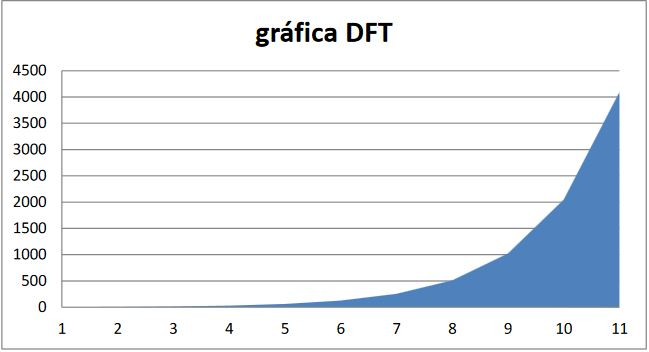
\includegraphics[width=0.8\textwidth]{imgDFT}
  \caption{Ejecución del programa.}
  \label{fig:FFT_1d}
\end{figure}

\begin{figure}[ht!]
  \centering
  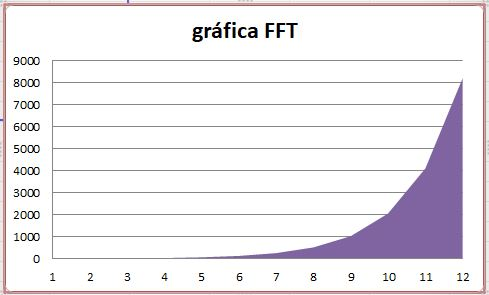
\includegraphics[width=0.8\textwidth]{imgFFT}
  \caption{Ejecución del programa.}
  \label{fig:FFT_1d}
\end{figure}


\\

\\

\section{Conclusiones.}
La Tramsformada Discreta de Fourier es util para el an\'alisis de señales de tiempo discreto y dominio finito pero resulta muy ineficiente al tratar con muestras grandes y por ello es indicado utilizar FFT el cual es exageradamente mas eficiente que el DFT.

\appendix
\section{Código fuente del Ejercicio 1.} 
\label{code:pendiente}

% Cuerpo
\begin{lstlisting}[language=C++]
#include <complex>
#include <iostream>
#include <valarray>
#include <time.h>
#include<fstream> 

using namespace std;


int n = 0;

//se utilizo complex
typedef complex<double> Complex;

typedef valarray<Complex> CArray;


double funcion(double);


template <class TI>
void obtener_datos(TI data[])
{
    for (int i = 0; i < n; i++)
    {
        data[i] = funcion(i);
    }
}

// la función DFT.
void DFT(CArray &, Complex[]);

int main()
{
    cout << "El numero maximo n = " ;
    int p;
    cin >> p;
    fstream myfile;
    myfile.open("DFT_I.txt", fstream::out);
    clock_t t;
    for (int j = 4; j <= p; j *=2)
    
    {
        n = j;
        Complex *test = new Complex[n];
        obtener_datos(test);
        CArray data(test, n);
        t = clock();
        DFT(data, test);
        t = clock() - t;
        cout << "n = " << n << "  ,  t = " << ((float)t) / CLOCKS_PER_SEC << endl;
        myfile << "{" << n << ", " << ((float)t) / CLOCKS_PER_SEC << " } , ";
        delete []test;
    }
    myfile.close();

    return 0;
}

double funcion(double x)
{
    return 2 * sin(2 * M_PI / n * x) + 5 * cos(2 * M_PI / n * x);
}


void DFT(CArray &x, Complex test[])
{
   
    for (int i = 0; i < n; i++)
    {
        double suma_R = 0;
        double suma_i = 0;
        for (int k = 0; k < n; k++)
        {
            suma_R += test[k].real() * cos(2 * M_PI / n * k * i);
            suma_i -= test[k].real() * sin(2 * M_PI / n * k * i);
        }
        x[i].real(suma_R);
        x[i].imag(suma_i);
    }
}

\end{lstlisting}

\section{Código fuente del Ejercicio 2.} 
\label{code:pendiente}

% Cuerpo
\begin{lstlisting}[language=C++]
#include <complex>
#include <iostream>
#include <valarray>
#include <time.h>
#include <fstream>

using namespace std;

int n = 8;


typedef complex<double> Complex;

typedef valarray<Complex> CArray;

double funcion(double);


template <class T>  //identificador de tipo: T
void obtener_datos(T data[])
{
    for (int i = 0; i < n; i++)
    {
        data[i] = funcion(i);
    }
}


void FFT(CArray &);

int main()
{
    cout << "num. maximo n = " ;
    long long int NN;
    cin >> NN;
    fstream myfile;
    myfile.open("FFT.txt", fstream::out);
    clock_t t;

    for (long int j = 4; j <= NN; j *= 2)
    {
        n = j;
        Complex *test = new Complex[n];
        obtener_datos(test);
        CArray data(test, n);

        t = clock();
        FFT(data);
        t = clock() - t;
cout << "n = " << n << "  ,  t = " << ((float)t) / CLOCKS_PER_SEC << endl;
myfile << "{" << n << ", " << ((float)t) / CLOCKS_PER_SEC << " } , ";
        delete []test;
    }
    myfile.close();

    return 0;
}


double funcion(double x)
{
    return 2 * sin(2 * M_PI / n * x) + 5 * cos(2 * M_PI / n * x);
}

// Definimos la estructura de la funcion FFT.

void FFT(CArray &x)
{
    const size_t n = x.size();
    if (n <= 1)
        return;

    
    CArray even = x[slice(0, n / 2, 2)];
    CArray odd = x[slice(1, n / 2, 2)];

    // Recurcividad
    FFT(even);
    FFT(odd);

    // Combinamos
    for (size_t k = 0; k < n / 2; ++k)
    {
        Complex t = polar(1.0, -2 * M_PI * k / n) * odd[k];
        x[k] = even[k] + t;
        x[k + n / 2] = even[k] - t;
    }
}
\end{lstlisting}

\section*{Referencias}
[1]  Dra. María del Pilar Gómez, Procesamiento digital de señales, Coordinación de computación, Versión: 11 de Octubre 2017.\\

[2] Ana Martínez Manzano,  Transformada rápida de Fourier Implementación y algunas aplicaciones, Facultad de Matemáticas, 2018. \\

[3] Jimmy Alexander Cortés Osorio, Jairo Alberto Mendoza Vargas, José A. Muriel Escobar, “Alternativa al Análisis en Frecuencia de la FFT”, Universidad Tecnológica de Pereira. ISSN 0122-1701, No 44, Abril de 2010. \\

[4] URL: https://www.tutorialspoint.com/mfc/mfc_carray.htm (visitado 26/11/2020). \\

[5] URL: https://www.uv.es/diazj/complex.pdf (visitado 29/12/2020). \\

[6] URL: https://codingornot.com/cc-plantillas-templates-en-c (visitado 29/12/2020). \\

[7] URL: http://www.cplusplus.com/forum/beginner/91382/ (visitado 19/01/2020). \\

[8] URL: https://stackoverflow.com/questions/15231466/
    whats-the-difference-between-pi-and-m-pi-in-objc   (visitado 19/01/2020).




\end{document}